%%%%%%%%%%%%%%%%%%%%%%%%%%%%%%%%%%%%%%%%%%%%%%%%%%%%%%%%%%%%%%%%%%%%%%%%
%
% LensTractor Method Paper
%
%%%%%%%%%%%%%%%%%%%%%%%%%%%%%%%%%%%%%%%%%%%%%%%%%%%%%%%%%%%%%%%%%%%%%%%%

\documentclass[useAMS,usenatbib]{mn2e}
%% letterpaper
%% a4paper

% \voffset=-0.8in

% Packages:
% \input psfig.sty
\usepackage{xspace}
\usepackage{graphicx}

% Macros:
% Project stuff:
\def\panstarrs{{\sc PS1}\xspace}

% JOURNALS
\newcommand {\apj} {ApJ}
\newcommand {\apjl} {ApJL}
\newcommand {\apjs} {ApJS}
\newcommand {\mnras} {MNRAS}
\newcommand {\apss} {Ap \& SS}
\newcommand {\aap} {A\&A}
\newcommand {\aj} {AJ}
\newcommand {\prd} {Phys. Rev. D}
\newcommand {\nat} {Nature}
\newcommand {\araa} {ARA\&A}
\newcommand {\jgr} {J. Geophys. Res.}
\newcommand {\pasp} {PASP}

% MISC
\newcommand {\etal} {et~al.~}
\def \spose#1{\hbox  to 0pt{#1\hss}}  
\newcommand {\lta} {\mathrel{\spose{\lower 3pt\hbox{$\sim$}}\raise  2.0pt\hbox{$<$}}}
\newcommand {\gta} {\mathrel{\spose{\lower  3pt\hbox{$\sim$}}\raise 2.0pt\hbox{$>$}}}
\def \ion#1#2{#1{\footnotesize{#2}}\relax}
\newcommand {\ha}  {\ifmmode H\alpha \else H$\alpha $ \fi} 
\newcommand {\hi} {\ion{H}{I} } 
% \newcommand {\Sref} {\S}
\def\Sref#1{Section~\ref{#1}\xspace}
\def\Fref#1{Figure~\ref{#1}\xspace}
\def\Tref#1{Table~\ref{#1}\xspace}
\def\Eref#1{Equation~\ref{#1}\xspace}
\def\Eqref#1{Eq.~(\ref{#1})\xspace}

% UNITS
\newcommand {\kms} {\ifmmode  \,\rm km\,s^{-1} \else $\,\rm km\,s^{-1}  $ \fi }
\newcommand {\kpc} {\ifmmode  {\rm kpc}  \else ${\rm  kpc}$ \fi  }  
\newcommand {\pc} {\ifmmode  {\rm pc}  \else ${\rm pc}$ \fi  }  
\newcommand {\Msun} {\ifmmode {\rm M_{\odot}} \else ${\rm M_{\odot}}$ \fi} 
\newcommand {\Zsun} {\ifmmode {\rm Z_{\odot}} \else ${\rm Z_{\odot}}$ \fi} 
\newcommand {\yr} {\ifmmode yr^{-1} \else $yr^{-1}$ \fi} 
\newcommand {\hMsun} {\ifmmode h^{-1}\,\rm M_{\odot} \else $h^{-1}\,\rm M_{\odot}$ \fi}

% COSMOLOGY
%\newcommand {\LCDM} {\ifmmode \Lambda{\rm CDM} \else $\Lambda{\rm CDM}$ \fi}

% LENSING
\def\zd{z_{\rm d}}
\def\zs{z_{\rm s}}
\def\zspdf{z_{\rm s,pdf}\;}
\def\Dd{D_{\rm d}}
\def\Ds{D_{\rm s}}
\def\Dds{D_{\rm ds}}
\def\Sigmacrit{\Sigma_{\rm crit}}
\def\REin{R_{\rm Ein}}
\def\MEin{M_{\rm Ein}}
\def\sigmasie{\sigma_{\mathrm{SIE}}}
\def\Mvir{M_{\rm vir}}
\def\Mhalo{M_{\rm h}}
\def\Vhalo{V_{\rm c,h}}
\def\rhalo{r_{\rm c,h}}
\def\qhalo{q_{3,\rm h}}
\def\vc{V_{\rm c}}
\def\rc{r_{\rm c}}
\def\q3{q_{3}}
\def\bsis{b_{\rm SIS}}

% SED/PHOTOMETRIC FITTING
\def\Mstar{M_{*}}
\def\logMstar{\log_{10}\left(\Mstar/\Msun\right)}
\def\Mstarb{M_{*,\rm b}}
\def\logMstarb{\log_{10}\left(\Mstarb/\Msun\right)}
\def\Mstard{M_{*,\rm d}}
\def\logMstard{\log_{10}\left(\Mstard/\Msun\right)}
% \def\Reff{R_{\rm eff}}
% \def\Reffb{R_{\rm eff,b}}
% \def\Reffd{R_{\rm eff,d}}
\def\Reff{R_{\rm 50}}
\def\Reffb{R_{\rm 50,b}}
\def\Reffd{R_{\rm 50,d}}
\def\sersic{S\'ersic}
\def\nb{n_{\rm b}}
\def\qb{q_{\rm b}}
\def\phib{phi_{\rm b}}
\def\nd{n_{\rm d}}
\def\qd{q_{\rm d}}
\def\phid{phi_{\rm d}}

% SOFTWARE/HARDWARE
\def\SExtractor{{\sc SExtractor}\xspace}
\def\hst{{\it HST}\xspace}
\def\acs{\hst/ACS\xspace}
\def\galfit{{\sc galfit}\xspace}
\def\idl{{\sc idl}\xspace}
\def\python{{\sc python}\xspace}
\def\SPASMOID{{\sc SPASMOID}\xspace}

% FILTERS
\def\Bfilter{F450W\xspace}
\def\Vfilter{F606W\xspace}
\def\Ifilter{F814W\xspace}
\def\Kfilter{K'\xspace}
\def\Bband{\Bfilter-band\xspace}
\def\Vband{\Vfilter-band\xspace}
\def\Iband{\Ifilter-band\xspace}
\def\Kband{\Kfilter-band\xspace}

% PROBABILITY THEORY
\def\pr{{\rm Pr}}
\def\data{{\mathbf{d}}}
\def\datap{{\mathbf{d}^{\rm p}}}
\def\datai{d_i}
\def\datapi{d^{\rm p}_i}
\def\masspars{\boldsymbol{\theta}_{\rm m}}
\def\srcpars{\boldsymbol{\theta}_{\rm s}}
\def\vrot{{\mathbf{v}}}
\def\vrotp{{\mathbf{v}^{\rm p}}}
\def\vrotmodel{\hat{\mathbf{v}}}
\def\vrotj{v_j}
\def\vrotpj{v^{\rm p}_j}

% SPECTROSCOPY
\def\Angstrom{A\xspace}
\def\CaII{Ca\,{\sc ii}\xspace}
\def\NaII{Na\,{\sc ii}\xspace}
\def\NaD{Na\,{\sc D}\xspace} % ??
\def\NII{N\,{\sc ii}\xspace}
\def\HeII{He\,{\sc ii}\xspace}
%\def\Mgb{Mg\,{\sc ii}} Mg II is something else, at 2800 A no?
\def\Mgb{Mg\,{\rm b}\xspace}
\def\Ha{H$\alpha$\xspace}
\def\Hb{H$\beta$\xspace}
\def\OII{[O\,{\sc ii}]\xspace}
\def\OIII{O\,{\sc iii}]\xspace}
\def\CIII{C\,{\sc iii}]\xspace}
\def\CIV{C\,{\sc iv}\xspace}
\def\FeII{[Fe\,{\sc ii}]\xspace}
\def\sigmap{$\sigma_{\rm ap}$}
\def\sigmasdss{$\sigma_{\rm SDSS}$}

% PAPER SERIES
\def\paperI{{Paper~I}\xspace}
\def\paperIfirsttime{{Treu \etal submitted, referred to hereafter as \paperI}\xspace}
\def\paperII{{Paper~II}\xspace}
\def\paperIIfirsttime{{Dutton \etal submitted, referred to hereafter as \paperII}\xspace}
\def\paperIII{{Paper~III}\xspace}
\def\paperIIIfirsttime{{Brewer \etal submitted, referred to hereafter as \paperIII}\xspace}

% SAMPLE PROPERTIES
\def\NSWELLS{27}
\def\NSWELLSNEW{19}
\def\NSWELLSHST{16}
\def\NSWELLSAO{3}
\def\NSWELLSA{8}
\def\NSWELLSB{1}
\def\NSWELLSC{6}
\def\NSWELLSX{4}
%10 spirals from slacs, including 8 ``edge-on''
\def\NSSLACS{10}
\def\NSESLACS{8}
\def\NTOTALA{16}

% COMMENTING
\usepackage[usenames]{color}
\newcommand{\aaron}[1]{\textcolor{Brown}{\bf #1}}
\newcommand{\phil}[1]{\textcolor{blue}{\bf #1}}
\newcommand{\brendon}[1]{\textcolor{Violet}{\bf #1}}
\newcommand{\tommaso}[1]{\textcolor{green}{\bf #1}}
\newcommand{\matt}[1]{\textcolor{orange}{\bf #1}}
\newcommand{\matteo}[1]{\textcolor{Magenta}{\bf #1}}
\newcommand{\flag}[1]{\textcolor{red}{\bf #1}}
\newcommand{\achtung}[2]{\textcolor{red}{\it\bf ATTENTION #1! #2}}

\def\kipac{Kavli Institute for Particle Astrophysics and Cosmology, Stanford University, 452 Lomita Mall, Stanford, CA 94035, USA}
\def\oxford{Department of Physics, University of Oxford, Keble Road, Oxford, OX1 3RH, UK}
\def\nyu{NYU}
\def\cmu{CMU}
\def\mpia{MPIA}
\def\ucsb{UCSB}

\def\pjmemail{\tt dr.phil.marshall@gmail.com}


%%%%%%% RESULTS %%%%%%%%%

%%%%%%%%%%%%%%%%%%%%%%%%%

%%%%%%%%%%%%%%%%%%%%%%%%%%%%%%%%%%%%%%%%%%%%%%%%%%%%%%%%%%%%%%%%%%%%%%%%

\title[Finding lensed quasars]
{Detecting strongly lensed quasars by pixel-level model comparison}

\author[]{%
  Philip J. Marshall$^{1,2}$\thanks{\pjmemail},
  David W. Hogg$^{3,4}$,
  Adriano Agnello$^{5}$,
  Dustin Lang$^{6}$,
  Eric P. Morganson$^{4}$,
  and others 
  \medskip\\
  $^1$\kipac\\
  $^2$\oxford\\
  $^3$\nyu\\
  $^4$\mpia\\
  $^4$\ucsb\\
  $^6$\cmu
}

%%%%%%%%%%%%%%%%%%%%%%%%%%%%%%%%%%%%%%%%%%%%%%%%%%%%%%%%%%%%%%%%%%%%%%%%

\begin{document}
             
\date{to be submitted to MNRAS}
             
\pagerange{\pageref{firstpage}--\pageref{lastpage}}\pubyear{2010}

\maketitle           

\label{firstpage}

%%%%%%%%%%%%%%%%%%%%%%%%%%%%%%%%%%%%%%%%%%%%%%%%%%%%%%%%%%%%%%%%%%%%%%%%

\begin{abstract}
In some heuristic sense, we will end up believing that a particular
astronomical source is a galaxy-scale strong gravitational lens only if it
is more plausible to explain it as a superposition of a gravitationally
distorted background source and a foreground lensing galaxy than it is to
explain it as a single object with very odd morphology. The automated
detection of strong gravitational lenses must involve consideration of
these plausbilities.
%
We investigate the explicit implementation of this principle in practice,
in the context of automated searches for lensed quasars in optical imaging
surveys. We construct a quantitative approximation to this comparison of
plausibilities by fitting multi-epoch, multi-band ground-based imaging of
gravitational lens candidates with two image models, one of which,
``Lens,'' is a point source being lensed by a simple model massive galaxy,
and the other is a complex ``Nebula'' constructed from a simple galaxy and
$K$ point sources.  We \emph{approximate} the relative plausibility of the
lensing hypothesis with a likelihood ratio between these models, evaluated
at best-fit (that is, not marginalized), penalized by a simple factor
accounting for relative model freedom. \comment{PJM}{Other approximations
should be investigated!}
%
We fit these models and compute the relative lensing plausibility for 10
confirmed lensed quasars and 40 confirmed non-lenses from the SDSS Quasar
Lens Search (SQLS).  We find that we [can/cannot] confidently identify the
lenses and rule out the non-lenses with our plausibility criteria.  Even
though the plausibility calculation involves fitting highly parametrized
models of astronomical sources and the varying point-spread function in
many pixels of imaging, it can be calculated in seconds to minutes on
contemporary hardware; we comment on how this scales to ongoing lens
searches in various wide field imaging surveys.
\end{abstract}

% Full list of options at http://www.journals.uchicago.edu/ApJ/instruct.key.html

\begin{keywords}
  gravitational lensing
\end{keywords}

\setcounter{footnote}{1}

%%%%%%%%%%%%%%%%%%%%%%%%%%%%%%%%%%%%%%%%%%%%%%%%%%%%%%%%%%%%%%%%%%%%%%%%
%%  SECTION 1: INTRODUCTION
%%%%%%%%%%%%%%%%%%%%%%%%%%%%%%%%%%%%%%%%%%%%%%%%%%%%%%%%%%%%%%%%%%%%%%%%

\section{Introduction}
\label{sec:intro}

In this paper we ask the following questions:

\begin{enumerate}

\item Can an approximate lens plausibility be used to distinguish lenses from
non-lenses across a realistic sample of pre-selected targets, such as those
selected from the SDSS spectroscopic object catalog during the SQLS?

\item What challenges will be faced when attempting a similar computation in a
wide-field imaging survey covering thousands of square degrees and potentially
millions of targets? And with which further approximations might these be
approached?

\end{enumerate}



%%%%%%%%%%%%%%%%%%%%%%%%%%%%%%%%%%%%%%%%%%%%%%%%%%%%%%%%%%%%%%%%%%%%%%%%
%%  SECTION 2: MODELS AND INFERENCE
%%%%%%%%%%%%%%%%%%%%%%%%%%%%%%%%%%%%%%%%%%%%%%%%%%%%%%%%%%%%%%%%%%%%%%%%

\section{Models and Inference}
\label{sec:model}


%%%%%%%%%%%%%%%%%%%%%%%%%%%%%%%%%%%%%%%%%%%%%%%%%%%%%%%%%%%%%%%%%%%%%%%%
%%  SECTION 3: DATA
%%%%%%%%%%%%%%%%%%%%%%%%%%%%%%%%%%%%%%%%%%%%%%%%%%%%%%%%%%%%%%%%%%%%%%%%

\section{Example Dataset}
\label{sec:data:example}

As a simple first example, we consider the lensed quasar system H1413$+$117
\citep{H1413}, as observed three times during the PS1 $3\pi$ survey. We 
made 10-arcsecond postage stamp images from three frames taken over the
course of one year (MJDs  55377, 55664, 55755) in two filters ($r$ and
$z$). The image quality varies considerably between the three observing
epochs.

% \section{Test Dataset}
% \label{sec:data:example}


%%%%%%%%%%%%%%%%%%%%%%%%%%%%%%%%%%%%%%%%%%%%%%%%%%%%%%%%%%%%%%%%%%%%%%%%
%%  SECTION 4: RESULTS
%%%%%%%%%%%%%%%%%%%%%%%%%%%%%%%%%%%%%%%%%%%%%%%%%%%%%%%%%%%%%%%%%%%%%%%%

\section{Results}
\label{sec:results}

\subsection{sec:results:example}

We first illustrate the operation of \LT with a sequence of plots generated
by the code. In \Fref{fig:H1413example-progress}, we show the Nebula4 model
fit just before the PSF parameters were unfrozen, in order to show the
impact of assuming a PSF model just based on the FWHM keyword in the image
headers. The model was initialized by hand, using ds9 to identify the image
positions.

%%%%%%%%%%%%%%%%%%%%%%%%%%
\begin{figure*}
\centerline{
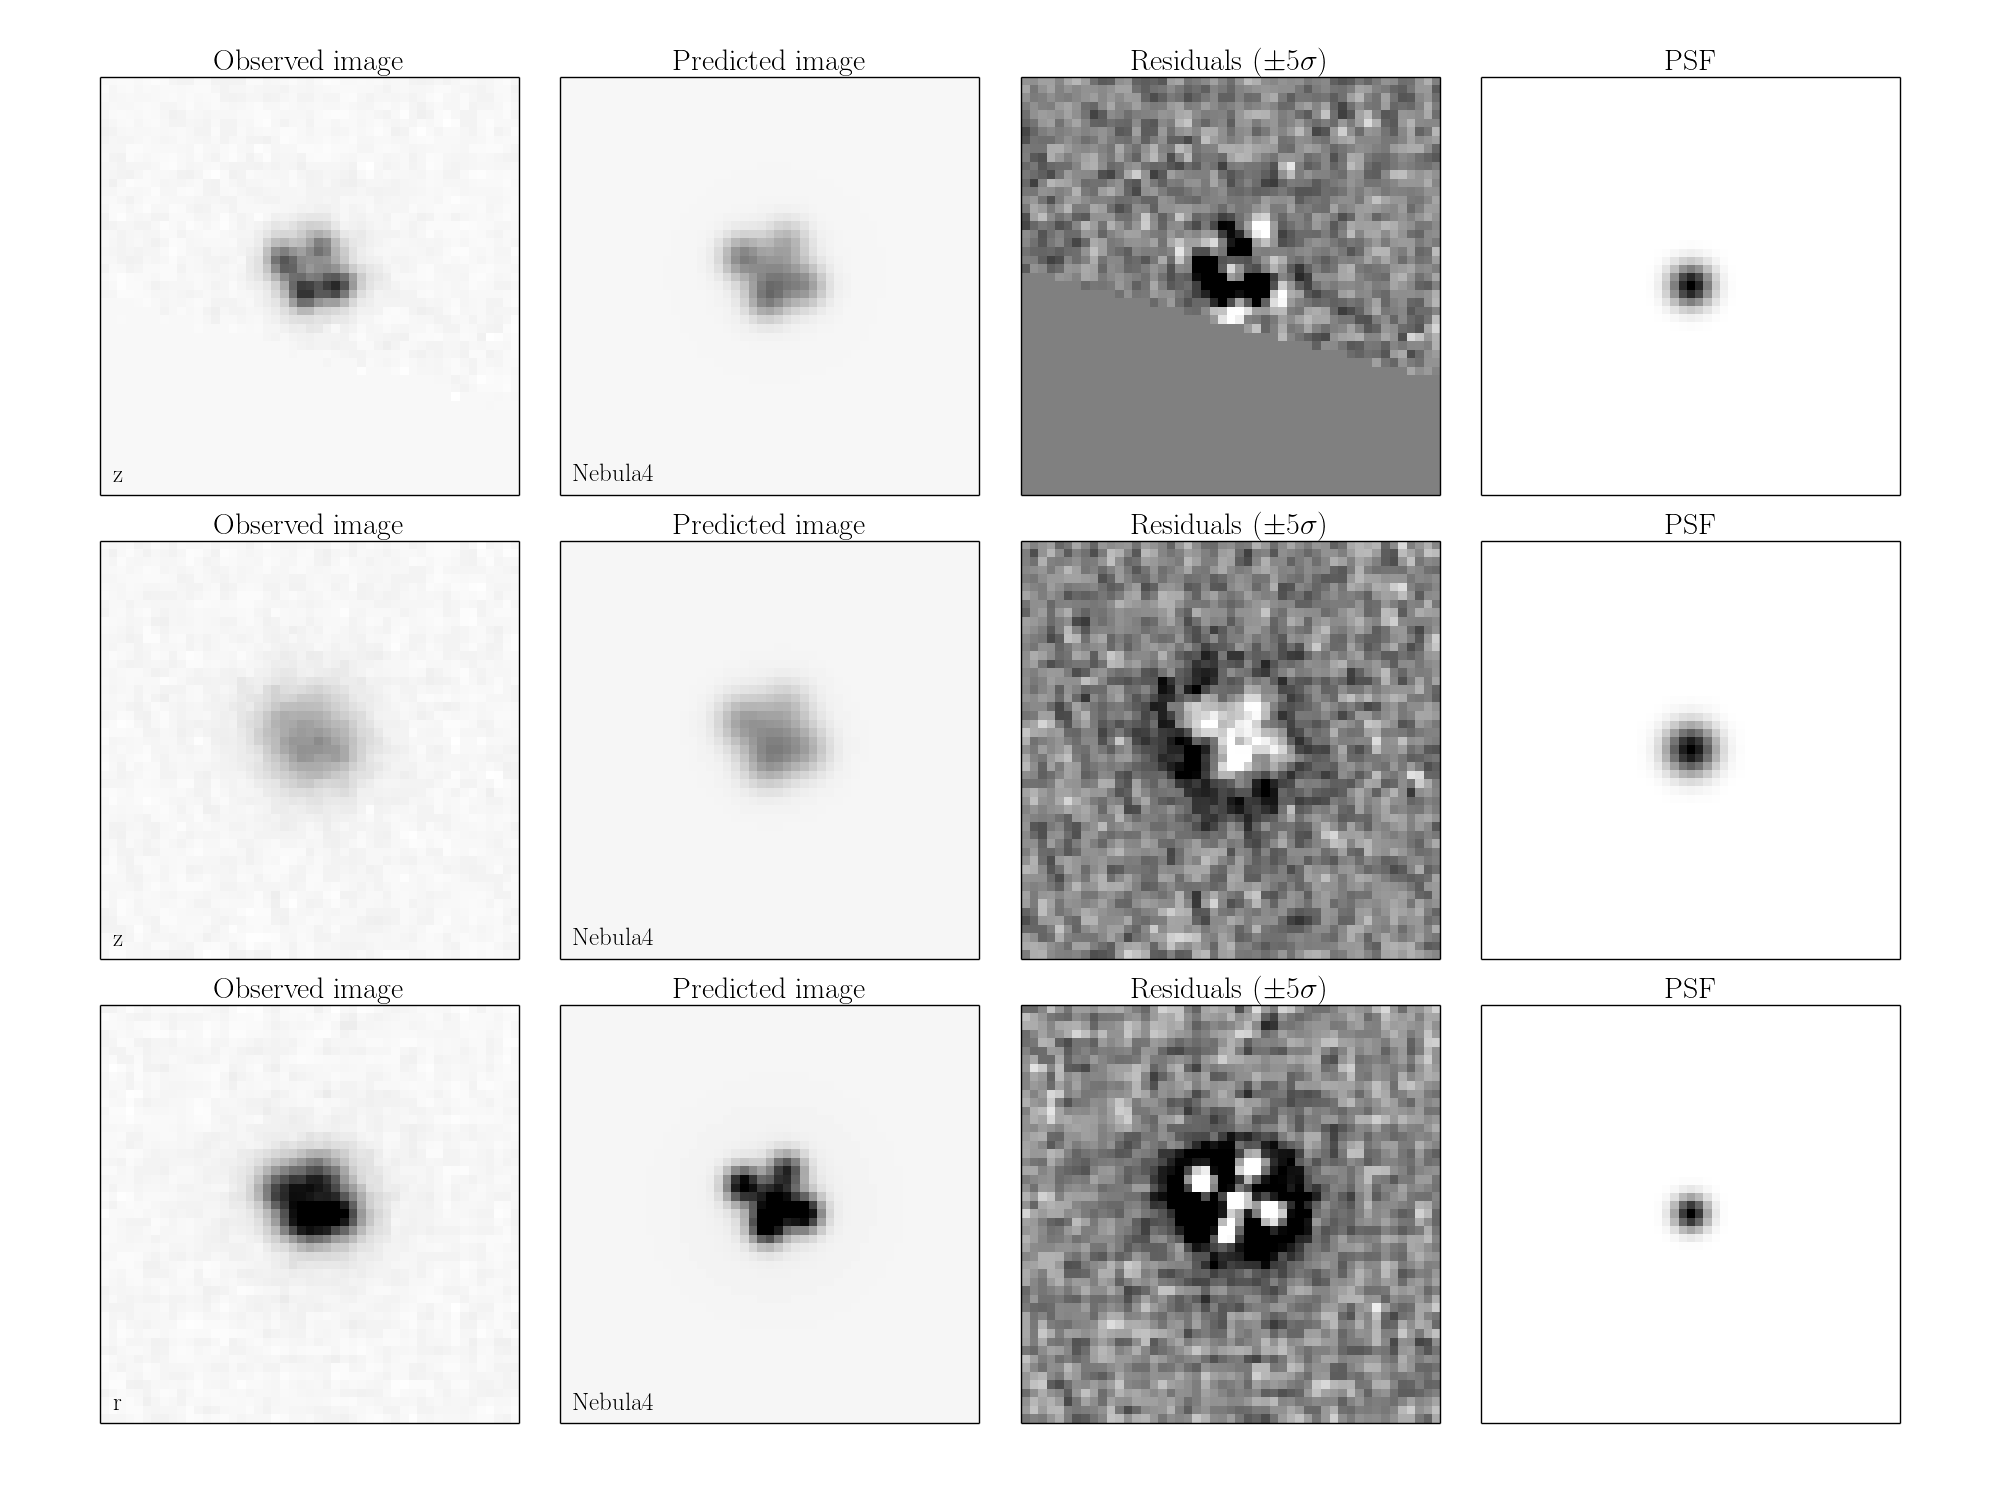
\includegraphics[width=0.9\linewidth]{figs/H1413+117_10x10arcsec_progress-06_optimizing_Nebula4.png}}
\caption{\LT example: three images of the known lens H1413+117, analyzed using
the Nebula4 model. This snapshot was taken mid-way through the inference, just
before the PSF parameters were unfrozen.}
\label{fig:H1413example-progress}
\end{figure*}
%%%%%%%%%%%%%%%%%%%%%%%%%%

\Fref{fig:H1413example-final} shows the final result of this fit, with both
the Nebula4 and PSF models optimized. The residuals are small but not
consistent with pure noise, suggesting either that the fit has not yet
converged, or that our simple model is not able to capture all the details
in the data, or both.

\action{PJM}{Add cartoon model overlays so we can check the fits.}

%%%%%%%%%%%%%%%%%%%%%%%%%%
\begin{figure*}
\centerline{
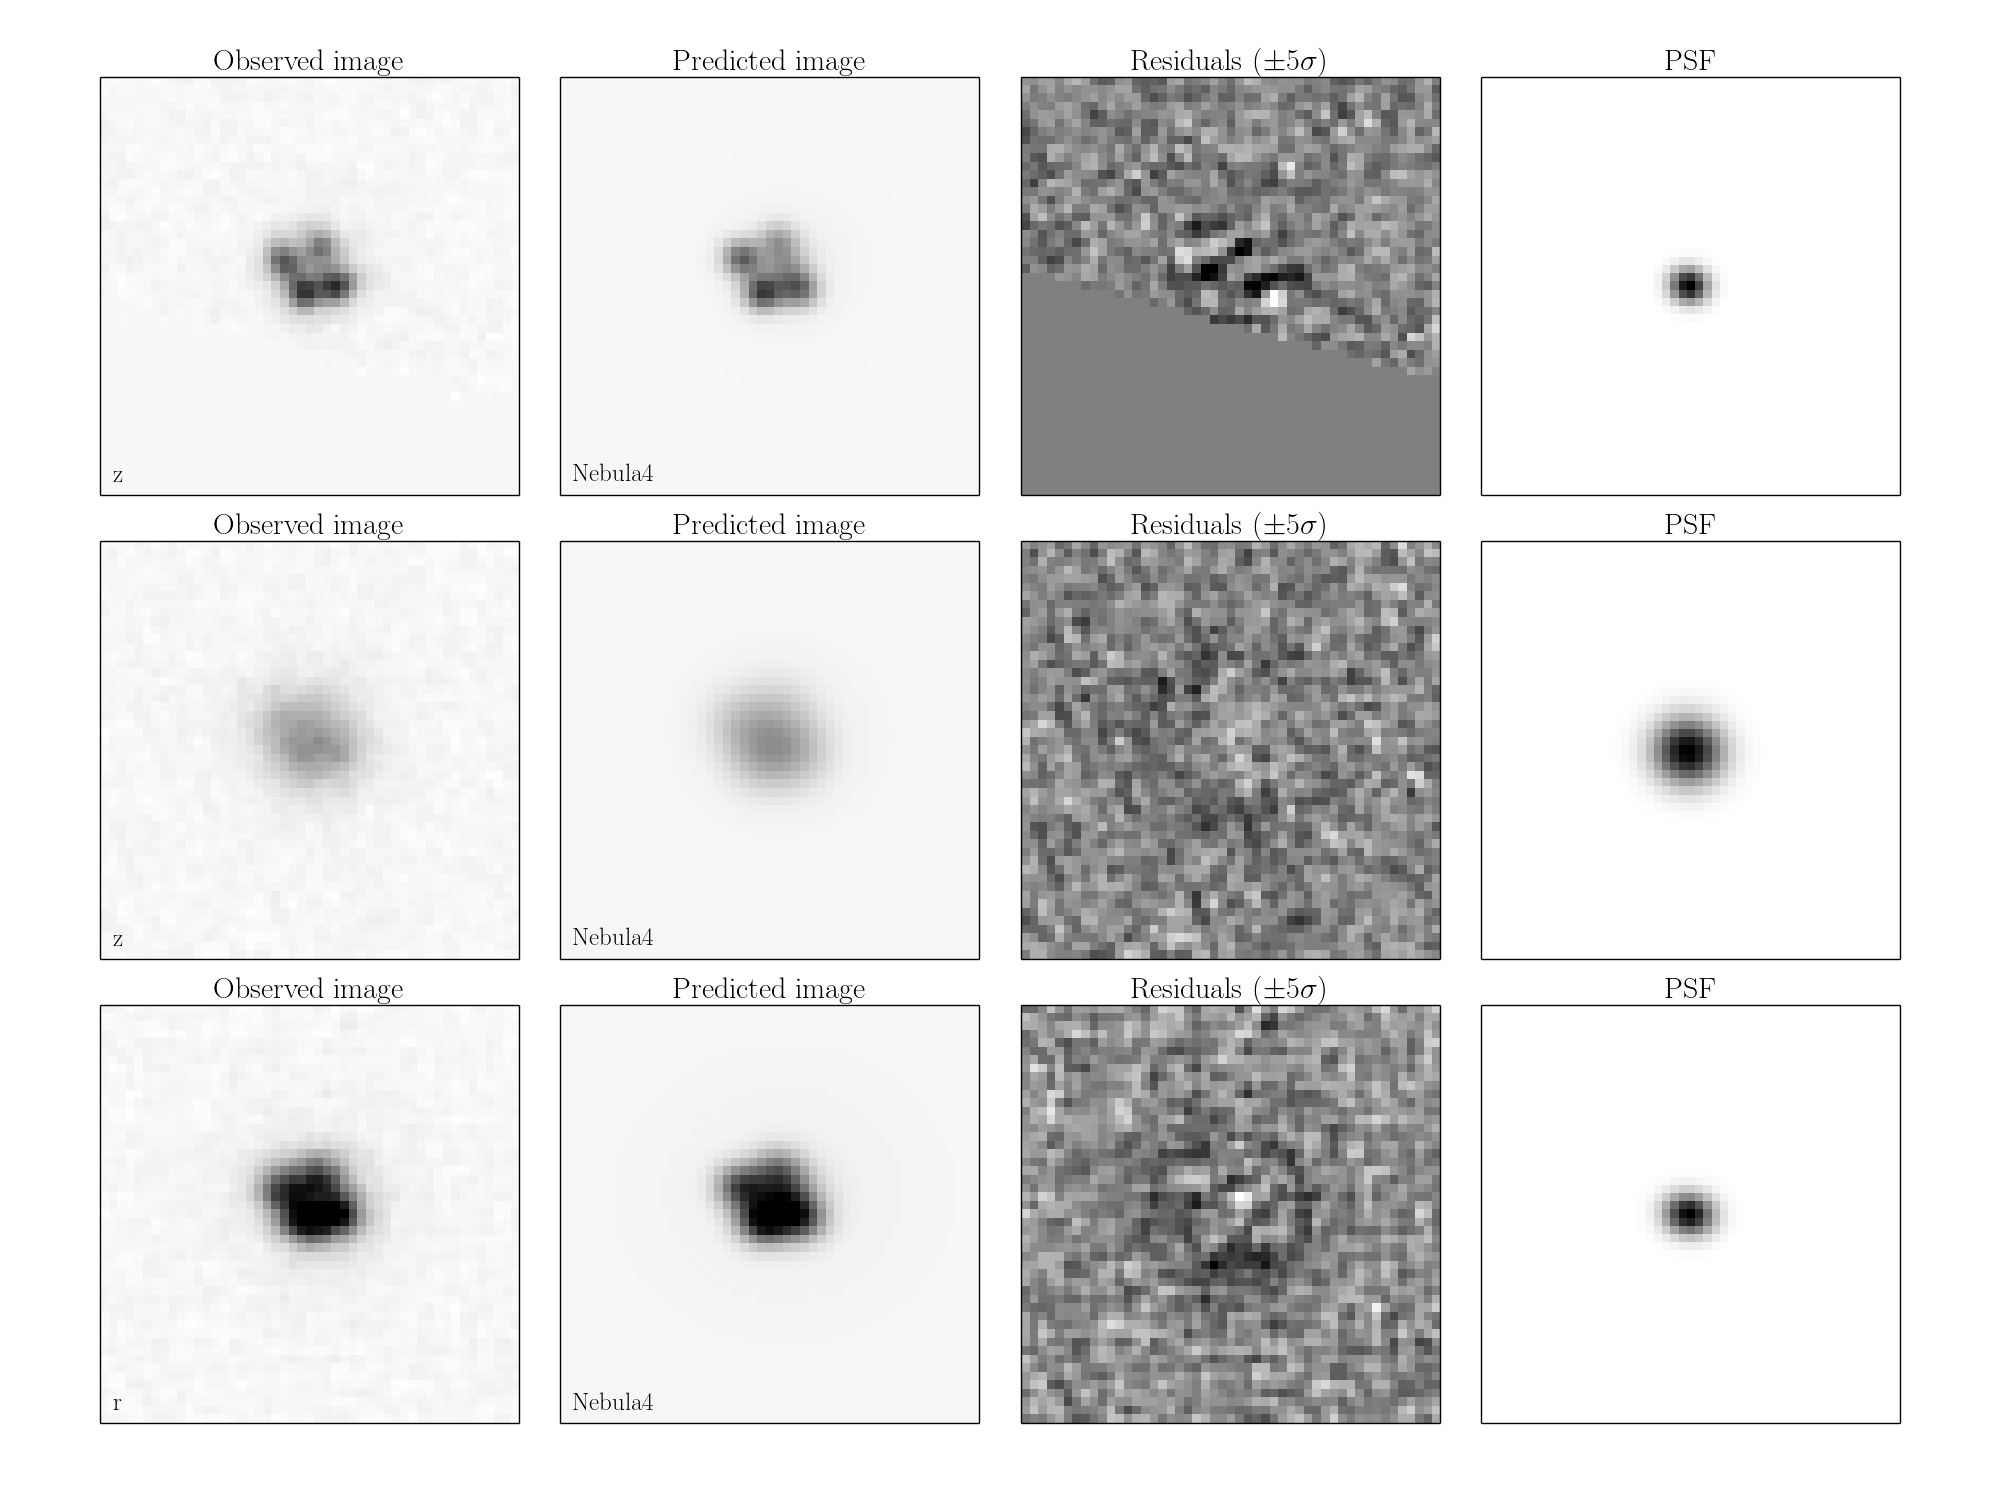
\includegraphics[width=0.9\linewidth]{figs/H1413+117_10x10arcsec_progress-09_optimizing_Nebula4.png}}
\caption{\LT example: the final result from the inference shown in
\Fref{fig:H1413example-progress}, with both the object and PSF models
optimized.}
\label{fig:H1413example-final}
\end{figure*}
%%%%%%%%%%%%%%%%%%%%%%%%%%

The performance of the Lens model initialization is quite sensitive to its
initialization. Ad-hoc placement of the model sources behind the 
model lens does not work reliably. Instead, we map the Nebula4 point source
positions back to the source plane through a lens with Einstein radius
estimated from the average separation between the Nebula4 point sources and
their mean position, and adjust the shear until the four corresponding
posint source positions match as closely as possible. Such a ``source plane
minimisation'' is fast, and accurate enough to initialize the lens model
close to the peak of its likelihood function. 

\comment{PJM}{This is a hypothesis, to be tested.}

\action{PJM}{Implement this Lens intialization.}


%%%%%%%%%%%%%%%%%%%%%%%%%%%%%%%%%%%%%%%%%%%%%%%%%%%%%%%%%%%%%%%%%%%%%%%%
%%  SECTION 5: CONCLUSIONS
%%%%%%%%%%%%%%%%%%%%%%%%%%%%%%%%%%%%%%%%%%%%%%%%%%%%%%%%%%%%%%%%%%%%%%%%

\section{Conclusions}
\label{sec:concl}

Our main results can be summarised as follows:

\begin{enumerate}

\item We now understand this.

\item And that.

\end{enumerate}


% do these comment headers really help?
% after all, the \section{} commands say THE SAME THING
% PJM: Yes, they break up the text in the editor, making it easier to navigate
% through a long file.
%%%%%%%%%%%%%%%%%%%%%%%%%%%%%%%%%%%%%%%%%%%%%%%%%%%%%%%%%%%%%%%%%%%%%%%%
%%  ACKNOWLEDGMENTS
%%%%%%%%%%%%%%%%%%%%%%%%%%%%%%%%%%%%%%%%%%%%%%%%%%%%%%%%%%%%%%%%%%%%%%%%

\section*{Acknowledgments}
 
We thank Sherry Suyu and James H.\ H.\ Chan, and Matt Auger and the STRIDES
collaboration for useful discussions and suggestions.
PJM acknowledges support from grants\ldots
DWH acknowledges support from grants\ldots

PJM was given support by the Royal 
Society, in the form of a research fellowship.
%
DWH ...
%
DL ...
%
% PS1



%%%%%%%%%%%%%%%%%%%%%%%%%%%%%%%%%%%%%%%%%%%%%%%%%%%%%%%%%%%%%%%%%%%%%%%%
%%  REFERENCES
%%%%%%%%%%%%%%%%%%%%%%%%%%%%%%%%%%%%%%%%%%%%%%%%%%%%%%%%%%%%%%%%%%%%%%%%

% MNRAS does not use bibtex, input .bbl file instead. 
% Generate this in the makefile using bubble script in scriptutils:

%   bubble -f swells-survey.tex references.bib 

\bibliographystyle{apj}
\bibliography{references}

%%%%%%%%%%%%%%%%%%%%%%%%%%%%%%%%%%%%%%%%%%%%%%%%%%%%%%%%%%%%%%%%%%%%%%%%

\label{lastpage}
\bsp

\end{document}

%%%%%%%%%%%%%%%%%%%%%%%%%%%%%%%%%%%%%%%%%%%%%%%%%%%%%%%%%%%%%%%%%%%%%%%%
